\chapter{Background\\(READY FOR PROOFREAD)}
\label{chapter:background} 
In this chapter ...
\section{Electricity consumption of ICT equipments}
\label{section:ictequipment} 
ICT devices consume a significant amount of electricity. A survey conducted by Heddeghem et al.{\ }\cite{DBLP:journals/comcom/HeddeghemLLCPD14} shows the electricity consumption and growth trends of three classes of ICT equipment: personal computers, communication networks, and data centers. Personal computers include equipment such as desktop, laptop and external monitors. Communication networks includes residential network access equipments (such as WiFi routers and modems), network equipments used in offices (such as routers and switches) and telecom-operator network equipments (such as base stations, routers and optical amplification systems). Data-centers house storage and computing servers, communication network equipments, and power provisioning and cooling facilities.  In this classification there are overlaps, for instance, telcom operator can have office network equipments and data-centers. After carefully avoiding possible redundant measurements, the researchers estimated absolute electricity consumption and annual consumption growth rate of each category of equipments for the period 2007 and 2012. The results of the study show that the  the global electricity consumption share of personal computers is 1.6\%, communication networks is 1.7\%, and data centers is 1.4\%. The estimated annual growth rate of each category is 5\% for personal computers, 10\% for communication networks, and 4\% for data-centers. These growth rates are higher than that of the total global electricity consumption, which is 3\%. This trend signifies the need for energy saving research in all the three categories.

\section {Data-center and network electricity consumption}
\label{section:datacenter} 
In Section~\ref{section:ictequipment} we described data-center's global share in electricity consumption. In this section we describe the components involved within the data center itself.

Electricity consumption units with in a typical data-center can be classified into two broad groups \cite{DBLP:journals/comsur/DayarathnaWF16}: The first group is IT equipments (which includes computing servers, storage servers and networking components) and the other group is infrastructure facilities (which includes power provisioning, cooling and lighting components).

Figure~\ref{fig:datacenterenergy} \cite{DBLP:journals/comsur/DayarathnaWF16} shows the electricity consumption proportion of the data-center components. This value differs significantly from one data-center to another \cite{DBLP:series/synthesis/2013Barroso}, for instance, due to architectural difference\cite{DBLP:conf/eenergy/GyarmatiT10} or energy efficiency of the components. The infrastructure facility components take the large proportion (65\%) of the consumption. 
\begin{figure}[ht]
	\begin{center}
		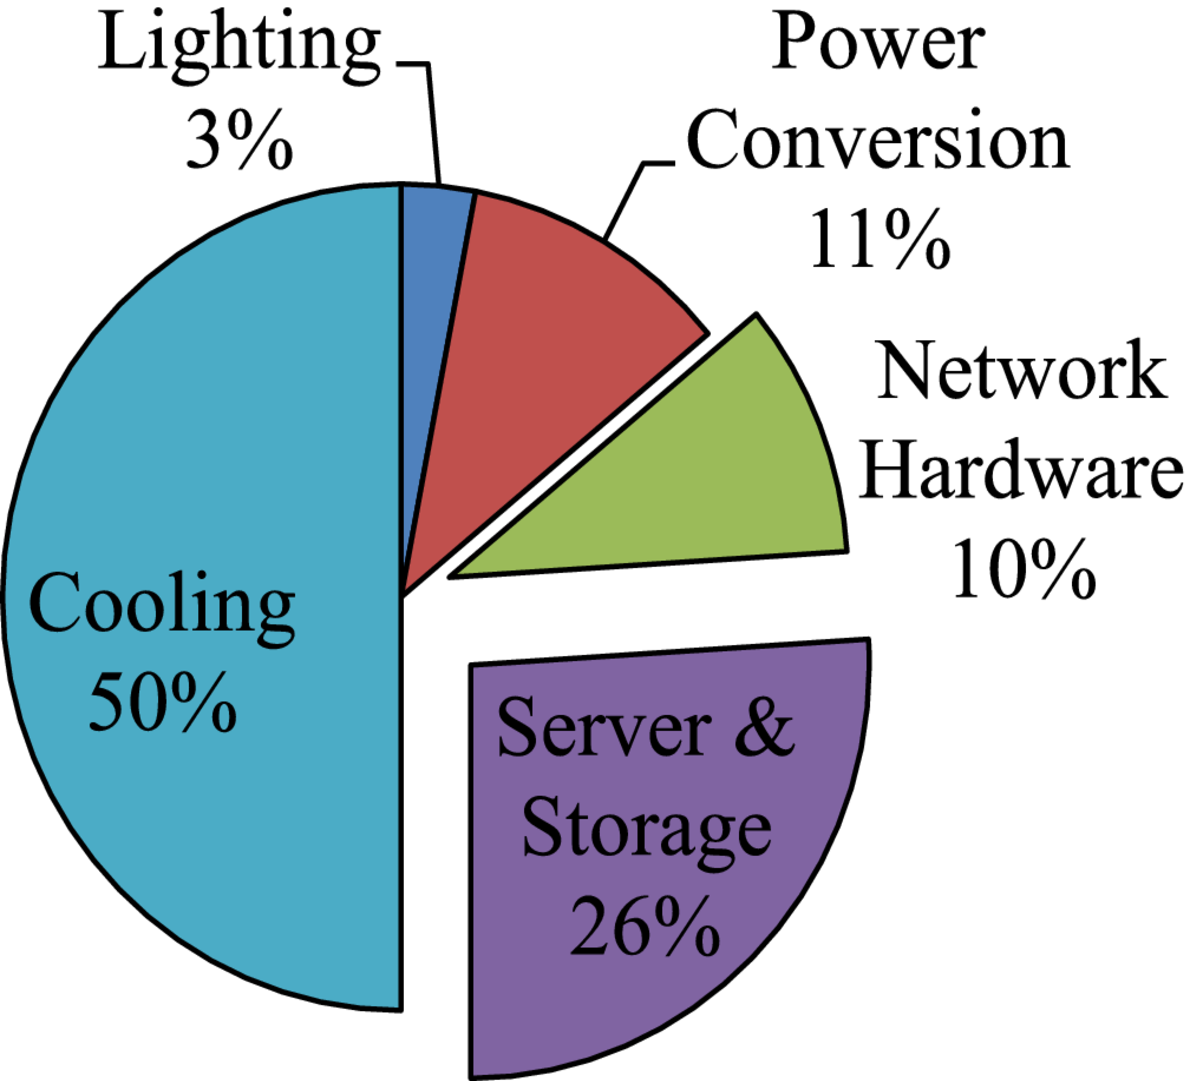
\includegraphics[width=7cm]{images/datacenterenergy.pdf}
		\caption{Energy consumption percentage of data-center components \cite{DBLP:journals/comsur/DayarathnaWF16}}
		\label{fig:datacenterenergy}
	\end{center}
\end{figure}
Though the infrastructure facility consumes relatively larger amount of electricity, the focus of this study is on the IT equipment components, particularly on the network equipment. 

If we further zoom in on the IT equipment part, we can find computing servers, storage servers and network devices. A data-center servers consist of one or more CPU cores, memory and I/O devices. The energy consumption relationship among these components is shown in Figure~\ref{fig:serverenergy}. Combined, Memory and CPU units consume the larger amount of energy relative to other components. The fact that CPU is the dominant electricity consuming unit is exploited by Fan et al. in \cite{DBLP:conf/isca/FanWB07} to model the dynamic power usage of thousands of servers by using only CPU utilization as a parameter. The result of their study was very accurate, with error as low as 1\%. The energy consumption contribution of storage servers in a typical data center is shown in Figure~\ref{fig:datacenterenergy} together with computing servers.
\begin{figure}[ht]
	\begin{center}
		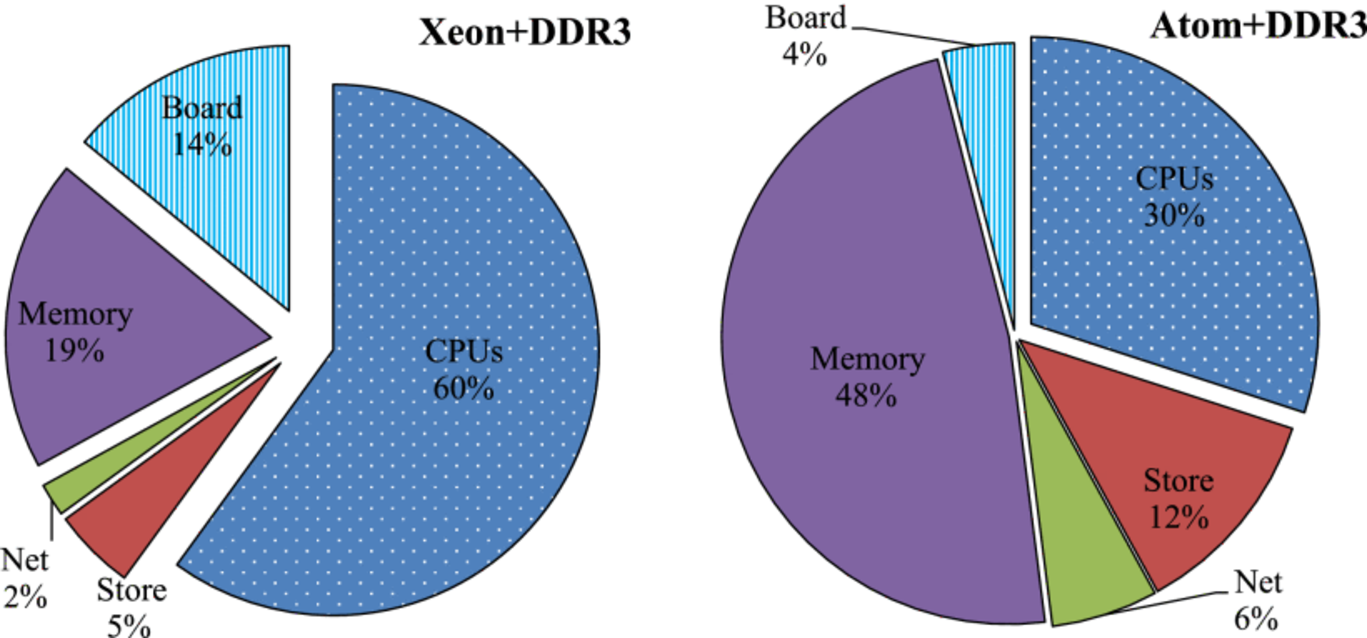
\includegraphics[width=11cm]{images/serverenergy.pdf}
		\caption{Energy consumption percentage of Xeon based (on the left) and Atom based (on the right) servers \cite{DBLP:journals/comsur/DayarathnaWF16}}
		\label{fig:serverenergy}
	\end{center}
\end{figure}

Network devices are the other part in the IT equipment component of a data center which contribute to energy consumption as shown in Figure~\ref{fig:datacenterenergy}. Shehabi et al.{\ }\cite{shehabi2016united}, from Berkeley National Laboratory, produced a report which show the annual energy consumption of network devices deployed in data centers residing in the United State. The historical and the forecast energy consumption is shown in Figure~\ref{fig:usnetworkenergy}. In the figure the energy consumption is grouped by port speed of 100Mbps, 1000Mbps, 10Gbps, and 40Gbps. 
\begin{figure}[ht]
	\begin{center}
		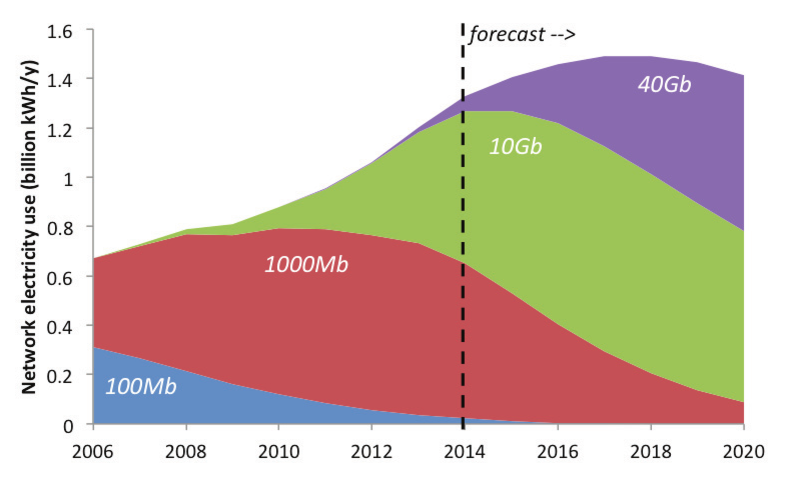
\includegraphics[width=11cm]{images/usnetworkenergy.pdf}
		\caption{Total data center network equipment energy consumption in the United States \cite{shehabi2016united}.}
		\label{fig:usnetworkenergy}
	\end{center}
\end{figure}

In large-scale distributed networks, network devices are deployed with in and outside the data center. Our study is not limited only to network devices residing in a particular data center, it also includes network devices residing outside a data center. 

\section{Energy proportionality}
\label{section:energyproportionality}
The primary reason the study of energy consumption management of network equipment becomes so important is that, in general, ICT equipments do not consume energy proportional to their workload. An ideal ICT equipment is the one which consume zero electricity when it is idle, and it consumes electricity proportional to its workload when it is active. However, the reality is, even power efficient servers consume about 50\% of their peak power \cite{DBLP:journals/computer/BarrosoH07}, even when they are doing nothing. This percentage can even reach 85\% for network switches \cite{DBLP:conf/IEEEcloud/FiandrinoKBZ15}. Figure~\ref{fig:energyproportionality} in \cite{DBLP:conf/networking/MahadevanSBR09} shows the energy proportionality of a typical network equipment. From the graph we can observe that the dynamic power consumption range is narrow.
\begin{figure}[ht]
	\begin{center}
		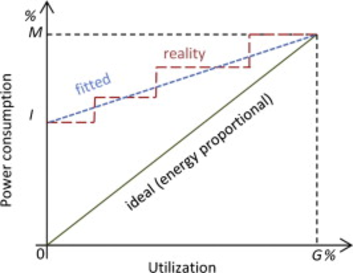
\includegraphics[width=11cm]{images/energyproportionality.pdf}
		\caption{Ideal and measured energy proportionality of a network equipment \cite{DBLP:conf/networking/MahadevanSBR09}}
		\label{fig:energyproportionality}
	\end{center}
\end{figure}
Three approaches are in common use to deal with this situation. The first one is re-engineering network devices so as to make them more energy proportional, device vendors are the prime role player in this aspect. The second approach is related to the operating rate of a network equipment port. A typical switch can operate on different transmission rate (100Mbps, 1 Gbps or 10 Gbps). An active port transmitting at 10 Gbps can consume more energy than if it transmit at 100 Mbps. Rate adaptation is the approach devised to take advantage of this situation. Instead of transmitting at the maximum rate all time,  the network port can be made to adapt to the actual traffic load. This energy saving approach is known as Adaptive Link Rate (ALR)\cite{DBLP:conf/nsdi/NedevschiPIRW08}. The third approach, which is known as Low Power Idle (LPI), allows a network device to send data as fast as possible and then enter low power mode between transfers \cite{DBLP:journals/computer/BarrosoH07}. The low power mode can further be extended by a technique called packet coalescing, which allows more energy saving \cite{DBLP:journals/comsur/BollaBDC11}. 
\section{Packet-level and flow-level Simulators}
\label{section:packetflow} 
One way of conducting experiment is to use real production environment or test-bed environment, both are referred to as \emph{in vivo} in \cite{DBLP:journals/jpdc/CasanovaGLQS14}. In the former case, handling transient and varying conditions would make the data collection and prediction very difficult and often times, a production environment is also not available for experimentation. In the later case, it requires setting-up a separate testing environment designed solely for the purpose of conducting the desired experiment. This approach apart from being expensive, it requires significant amount of time for experiment setup and, it is also non-repeatable as experimenting with different scenario demands a significantly modified or completely new configuration.

The other alternative for experimenting is simulation, also referred to as \emph{in silico} in \cite{DBLP:journals/jpdc/CasanovaGLQS14}. Simulation, unlike real environment, allows great flexibility in terms of experiment configuration, control and repetition. In addition it can also be less time consuming and less expensive.That is why virtually in all computer network related researches simulations are widely used. 

Simulators use models to specify the relationship between the variables involved in a particular network phenomenon. Generally, the models are classified as packet-level and flow-level models based on the detail of information the models are trying to capture. We can also refer to simulators as packet-level simulator and flow-level simulators based on the model they use. 

Packet-level simulators strives to model a given network phenomenon at the granularity level of individual packets. Due to the detail of information this simulators capture, in general, they are accepted by the research community to be more accurate compared to flow-level ones \cite{DBLP:journals/jpdc/CasanovaGLQS14}. One of the most popular packet-level simulator is NS-3, which is categorized under discrete-event simulator with events corresponding to sending and receiving of packets \cite{ns3}. Though packet-level simulators are accepted to be more accurate, they fail to scale well in the field of large-scale distributed networks due to the computation and storage cost involved in processing and storing each packet. 

In the area of large-scale networks, flow-level simulators are the preferred simulation alternative. Rather than modeling a given network phenomenon at an individual packet level, flow-level models treat a set of packets as a single unit \cite{DBLP:journals/jpdc/CasanovaGLQS14}. The most commonly used definition for flow in the context of computer networking is coined by Claffy et al.{\ }in \cite{claffy1998nature}: 

``\ldots a flow \ldots a unidirectional traffic stream with a unique [source-IP-address, source-port, destination-IP-address, destination-port, IP-protocol] tuple \ldots''

In addition to the five tuple mentioned in the definition, a flow also has a limited time duration. Claffy et al.{\ }\cite{claffy1998nature} used a time limit of 64 seconds as a flow duration in their study. Researchers such as Carneiro et al.{\ }\cite{DBLP:conf/valuetools/CarneiroFR09}, adopted this same definition to develop flow monitoring module for NS-3, a module that can generate information such as amount of packets or bytes transferred, packets dropped or transmission start and end time for each flow. Barakat et al. in \cite{DBLP:journals/tsp/BarakatTIDO03} also used the same definition to model traffic at the flow-level for the Internet backbone link. By abstracting away fine details, flow-level models provides easy way to instantiate experiments and they also scale very well for conducting large-scale network simulations \cite{DBLP:journals/jpdc/CasanovaGLQS14,DBLP:journals/tsp/BarakatTIDO03}.

The flow definition given above is not the only one. Any analytical model which capture the characteristics of a given network phenomenon can be considered as flow-level model. In SimGrid, for instance, TCP flow is characterized by bandwidth and end-to-end latency\cite{DBLP:journals/jpdc/CasanovaGLQS14}.
\section{Simulating and modeling energy consumption of large-scale networks}

In this study we simulate energy-aware large scale distributed networks using SimGrid (Detail description about SimGrid follows in the next section). When we say large-scale distributed network, we are referring to a set of networks residing inside in the distributed data centers and also the networks that are used to connect them. 

The energy consumption E of an equipment depends on the operating power P at time t. The total energy consumption for a time period T is given by Equation~\ref{eq:2.1} \cite{DBLP:conf/wowmom/OrgerieLLL11}. 
\begin{equation} \label{eq:2.1}
  E(T) = \int_{0}^{T} P(t) dt
\end{equation} 
Due to the energy proportionality characteristic described in Section~\ref{section:energyproportionality}, the common approach used to compute the energy consumption is to divide the power component into two parts: static/idle power (\($$P_{static}$$\)) and dynamic power (\($$P_{dynamic}$$\)) as shown in equation~\ref{eq:2.2}. Then the total energy is obtained by multiplying the total power, \($$P_{total}$$\) by the time duration \cite{DBLP:conf/wowmom/OrgerieLLL11,DBLP:journals/tjs/KliazovichBK12,DBLP:conf/networking/MahadevanSBR09,DBLP:journals/comsur/DayarathnaWF16}. 
\begin{equation} \label{eq:2.2}
 P_{total} = P_{static} + P_{dynamic}
\end{equation} 
For a typical network equipment such as a switch, the static part constitutes the power consumption of the chassis and the line-cards (when all the ports on the line-cards are switched off). The dynamic part, on the other hand, constitutes the power consumption of the switch ports running at a given rate multiplied by the utilization factor \cite{DBLP:conf/networking/MahadevanSBR09}. Equation~\ref{eq:2.3} shows how to compute the total power for a switch, where \($$P_{switch}$$\), is the total power consumption of a switch, \($$P_{chassis}$$\) and \($$P_{linecard}$$\) is the idle power consumption of the chassis and the line card, respectively. \($$P_{rate}$$\), is the power consumption of a given port at a given rate and \($$numports_{rate}$$\) is the number of ports running at a given rate. The rate can take values such as 10 Mbps, 100 Mbps, 1 Gbps or 10 Gbps.
\begin{equation} \label{eq:2.3}
\begin{split}
P_{switch} &= P_{chassis} + (numlinecards \times P_{linecard})  + \\
&\sum_{rate=min}^{max} (numports_{rate} \times P_{rate} \times utilizationFactor)
\end{split}
\end{equation}
\section{SimGrid}
\label{section:simgrid} 
SimGrid is one of the popular simulator available for simulating large-scale distributed networks such as grid, cloud, volunteer and HPC \cite{simgrid}. It employs flow-level models in its core for simulating different network resources and phenomenon. In subsequent paragraphs we give overview of its architecture, the pros and cons of the employed TCP flow-level model and its current status in relation to energy consumption simulation models.

Figure~\ref{fig:SimGrid} shows the structure of SimGrid and how its core works. The top three components are the APIs that users can use to develop their simulation. Both MSG and SMPI are used to specify simulated applications as concurrent processes. The difference is that using MSG, users can simulate any arbitrary application, whereas, using SMPI users can simulate existing MPI applications, the MPI processes are created automatically from C or Fortran MPI programs. SIMDAG, on the other hand, does not use concurrent processes. It allows users to describe their application as communicating task graph. The next layer, SIMIX, implements the mechanisms that are required to simulate the concurrent process of MSG and SMPI applications. It also provides process control and synchronization functionalities. The bottom layer, SURF, is the simulation core, it simulates the execution of activities on computing or communication resources \cite{DBLP:journals/jpdc/CasanovaGLQS14}.
\begin{figure}[ht]
	\begin{center}
		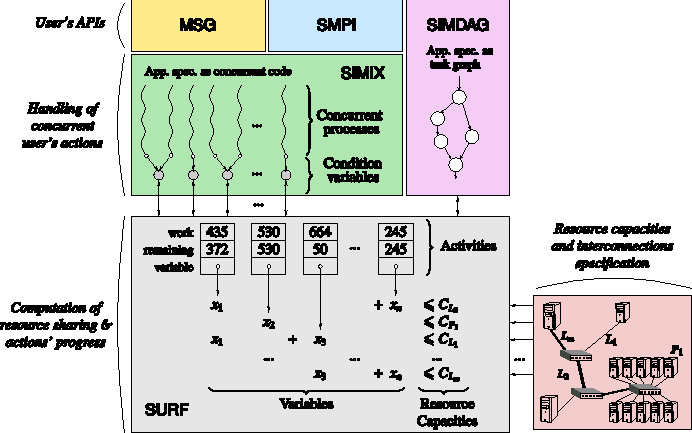
\includegraphics{images/SimGrid.pdf}
		\caption{Architecture of SimGrid \cite{DBLP:journals/jpdc/CasanovaGLQS14}}
		\label{fig:SimGrid}
	\end{center}
\end{figure}
In SimGrid for each simulated activity, such as computation or data transfer, there is a corresponding condition variable, in Figure~\ref{fig:SimGrid} it is shown in SIMIX box. This condition variable synchronizes the concurrent processes of the simulated applications. The computing (\($$P_{x}$$\)) and the communication (\($$L_{x}$$\)) resources are shown on the bottom-right side of the figure. Computing resources are defined in terms of computing power, whereas, communication resources are defined in terms of bandwidth and latency. As shown in the SURF box, multiple activities can share the same resource (e.g., (\($$x_{1}$$\), \($$x_{n}$$\)), (\($$x_{1}$$\), \($$x_{3}$$\)) or (\($$x_{3}$$\), \($$x_{n}$$\))) or one activity can use multiple resources (e.g., \($$x_{1}$$\) or \($$x_{3}$$\) or  \($$x_{n}$$\)). Activities that share the same resource are limited by the capacity of that resource. Each activity is defined by the total and remaining work to be executed. When the work associated with the activity completes, the corresponding upper layer components receive a notification signal \cite{DBLP:journals/jpdc/CasanovaGLQS14}.

As we have already pointed out in Section~\ref{section:packetflow}, the primary advantage of flow-level simulation is its scalability in terms of speed and memory usage. SimGrid uses flow-level analytical model for simulating TCP network phenomenon \cite{DBLP:journals/jpdc/CasanovaGLQS14}. To show the scalability of the flow-level model, the SimGrid team compared it with other widely used simulators such as GridSim and OverSim. After simulating 500,000 tasks both on GridSim and SimGrid, the results demonstrate that SimGrid is 257 times faster and 26 times more memory efficient. Similarly, the comparison result with OverSim shows that SimGrid is 15 times faster and it can also simulate scenarios 10 times larger. Concerning the accuracy, though the simulator gives very good accuracy in most case studies, there are situations where it fails to give accurate result. As an example, the comparison study of SimGrid with packet-level simulator GTNetS shows that for data size less than 100 KiB there is a significant difference in prediction. 

Currently, SimGrid has energy consumption model for CPU. Using this CPU model researchers can simulate energy consumption of single or multi core CPUs running at different operating frequencies. Concerning network equipment however, SimGrid has no energy consumption model. Therefore, the focus of this study is to propose and implement network energy consumption model for SimGrid. The implementation of this model, together with the existing CPU energy model, allows us to estimate the energy consumption of large-scale networks that reside within or outside a data-center such as networks discussed in Section~\ref{section:ictequipment} and Section~\ref{section:datacenter}.

\section{Related Simulators}
\label{section:relatedsimulator} 
In this section we review existing simulators that are proposed for estimating energy consumption of large-scale networks. 
\subsubsection{ECOFEN}
\label{subsection:ecofen} 
Orgerie et al.{\ }\cite{DBLP:conf/wowmom/OrgerieLLL11} proposed ECOFEN, an Energy Consumption
mOdel For End-to-end Networks. It is a packet-level simulator designed for estimating energy consumption of large-scale networks. Initially the simulator was developed as NS-2 module but currently it is also available as NS-3 module \cite{DBLP:conf/cloudnet/CorneaOL14}. ECOFEN provides three models for simulating energy consumption at different levels of granularity: \emph{basic}, \emph{linear} and \emph{complete}.

The basic model allows to simulate energy consumption of a network interface card (NIC) at coarse level of granularity. It only accept energy consumption value for ON and OFF state of the NIC. The linear model, on the other hand, accepts energy consumption value for the idle state of the NIC and for each bytes processed. This model allows to compute power consumption of a given network traffic. The complete model like the linear model also considers traffic in its power consumption computation. The difference is that it offers added flexibility in terms of parameters. Different energy consumption values can be assigned for bytes received or send and also packets received or send. All the three models produce the estimated average energy consumption at milliwatt precision level in the chosen time interval and the time interval can be set as small as a millisecond. 

ECOFEN module has two main limitations, mainly due to the limitation of the underlying NS-3 simulator. The first limitation comes from the lack of CPU abstraction in NS-3. As we have discussed in Section~\ref{section:datacenter}, server energy consumption is the second dominant part in typical data center and CPU is the main contributer among server parts such as memory and storage. Furthermore, since the energy consumption of CPU is linearly dependent on its operating frequency and its workload, the energy consumption increases more as the workload increases. As a consequence of absence of CPU from NS-3, the energy estimation we get from ECOFEN is partial. It only able to simulate energy consumption of network components such as NIC, switches and routers. The second limitation is concerned with the scalability issue. Being a packet-level simulator, the performance of ECOFEN is affected significantly as the number of processed packets grows large. Cornea et al.{\ }\cite{DBLP:conf/cloudnet/CorneaOL14} noticed this scalability problem during their study of the energy consumption of data transfers in clouds using ECOFEN module. It took them 5 hours to capture 1 minute of simulated network activity. 
\subsubsection{GreenCloud}
Kliazovich et al.{\ }\cite{DBLP:journals/tjs/KliazovichBK12} proposed GreenCloud, a simulator that can estimate energy consumption of cloud computing data centers. GreenCloud is developed as extension to NS-2 packet-level network simulator. This simulator contains power consumption models both for the computing and communicating components of a typical data center. The power consumption model used for the computing component is shown in Equation~\ref{eq:2.4}. This equation contains power consumed by the fixed parts (such as bus, memory and disk) which consume power independent of the operating frequency \emph{f} of the computing component CPU and the power consumed by the CPU (\($$P_f$$\)) operating at a given frequency \emph{f}. This model allows for lowering the operating frequency of the CPU when workload becomes below some predefined threshold in order to decrease the power consumption. 
\begin{equation} \label{eq:2.4}
P_{computing} = P_{fixed} + P_f \times f^3
\end{equation}h=
The power consumption model used in GreenCloud for the communicating components is the one shown in Equation~\ref{eq:2.3}. The equation shows the static power consuming parts (such as the chassis(\($$P_{chassis}$$\))and the active line cards(\($$P_{linecard}$$\)) and the dynamic part (\($$P_{rate}$$\)) is the energy consumed by the port running at a particular line rate for a given traffic load. 

This simulator is limited in four aspects: (1) in the number of allowed CPU cores, (2) in versatility, and (3) in scalability. The first limitation is that only one CPU core is allowed per simulated node. This hinders the study of energy consumption of multi-core computing nodes. The second one is that we can not use this simulator outside the cloud computing domain such as grid, volunteer, peer-to-peer or HPC, at least that is not the authors original intention when they develop this simulator. The available features of the simulators are tuned towards cloud computing applications only. This limits its versatility. The third limitation deals with the scalability issue. The fine grain details provided by GreenCloud and the packet-level processing approach of the underlying NS-2 simulator is advantageous for getting accurate result when simulating relatively small networks. However, for large-scale distributed networks, it is not scalable. In related to this, the authors have mentioned that the simulation speed gets slower and slower as the number of simulated nodes increases beyond few thousands and also as the number of processed packets increase. The GreenCloud's underlying simulator NS-2, is known for its scalability problem. Currently NS-3 is available as a better performing alternative \cite{DBLP:conf/icc/WeingartnerLW09} however, we could not find any upgraded for GreenCloud.





